\subsection{Der neuronale Multiplikator}
Mit der Einführung der Burgersgleichung wird nun ersichtlich, dass das neuronale Netzwerk unter anderem eine Multiplikation 'erlernen' muss. Die Multiplikation zweier Zahlen ($a \cdot b$) ist für uns einfach, jedoch ist dies für ein neuronales Netzwerk nicht so einfach. Ein KNN ist nicht in der Lage eine Multiplikation exakt zu erlernen, im Gegensatz zur Ableitung 2. Ordnung. Das erlernen bedeutet also eine Annäherung der Funktion. Die einfachste Netzwerktopologie entspricht der Abbildung \ref{fig:mst_simple_multiplicator}.

\begin{figure}[h]
	\centering
	\begin{tikzpicture}
	\node[inputNode, thick] (i1) at (-1, 0.5) {};
	\node[inputNode, thick] (i2) at (-1, -0.5) {};
	
	\node[inputNode, thick] (o1) at (1, 0.0) {};
	
	
	\draw[stateTransition] (-2, 0.5) -- node[above] {$I_1$} (i1);
	\draw[stateTransition] (-2, -0.5) -- node[above] {$I_2$} (i2);
	
	\draw[stateTransition] (i1) -- (o1);
	\draw[stateTransition] (i2) -- (o1);
	
	
	\draw[stateTransition] (o1) -- node[above] {$O_1$} (2, 0);
	\end{tikzpicture}
	\label{fig:mst_simple_multiplicator}
	\caption{Topologie des trivialen Multiplikators}
\end{figure}

Der triviale Multiplikator kann somit die Multiplikation mit der Form der Gleichung \ref{eq:mst_trivial_sum} annäheren. 

\begin{equation}
I_{1} \cdot I_{2} \; \hat{=} \; \sigma \left( \omega_{1} I_1 + \omega_{2} I_2 + b \right) 
\label{eq:mst_traivial_sum}
\end{equation}

Ein solches Gleichungssystem ist nicht befriedigend (auch mit Fehler) lösbar. Dies zeigt, dass mit $I_1 = I_2$ die Funktionsentwicklung einer quadratischen Funktion entspricht. Die Summe auf der rechten Seite ist ohne Aktivierungsfunktion linear. Selbst bei Verwendung von gängigen Aktivierungsfunktionen wie der Sigmoid- oder Tangens hyperbolicus Funktion kann keine gute Nähreung gefunden werden. 

Durch den Satz von Stone-Weierstrass ist bewiesen, dass jede stetige Funktion durch einfachere Funktionen beliebig gut auf einem Interval $[a, b]$ aproximiert werden kann. Mit dieser Erkenntnis und dem Konzept der Neuronen kann man folgende Gleichung aufstellen:

\begin{align}
I_{1} \cdot I_{2} \; & \hat{=} \; \sigma_{1} \left( \omega_{11} I_1 + \omega_{12} I_2 + b_{1} \right) + \sigma_{2} \left( \omega_{21} I_1 + \omega_{22} I_2 + b_{2}  \right) + \dots  + \sigma_{n} \left( \omega_{n1} I_1 + \omega_{n2} I_2 + b_{n} \right) \\
I_{1} \cdot I_{2} \; & \hat{=} \sum_{k=1}^{n} \sigma_{k} \left( \omega_{k1} I_1 + \omega_{k2} I_2 + b_{k} \right)
\label{eq:mst_traivial_sum}
\end{align}
 
Diese Gleichung lässt sich nun in ein neuronales Netzwerk mit einem hidden Layer übersetzten wie Abbildung \ref{fig:mst_variable_hidden_layer} zeigt. Es ist auch ersichtlich, dass die Aktivierungsfunktion des Outputlayers linear ist und dieser keine Bias-Variable $b_{out}$ besitzt. Der Einfachheit halber verwenden wir aber ein Gewicht $w_{2n}$ im Outputlayer für die Konstrution der Linearkombination.

Mit steigender Anzahl Neuronen sollte somit der Fehler. Um diese Hypothese zu bestätigen, wurde ein Netzwerk verwendet, welches gemäss der Abbildung \ref{fig:mst_variable_hidden_layer} implementiert wurde. Die Neuronen im hidden Layer sind variabel zwischen 2 und 14 gewählt und das Interval für $I_1$ und $I_2$ umfasst $[0, 10)$. Die Daten wurden mit Hilfe von 2 zufällig initialisierten Arrays erstellt. Die Zahlen sind diskretisiert in $0.1$ Schritten. Es existieren somit theoretisch 10000 Kombinationen, davon wurden 5000 Datenpunkte verwendet um die Netze zu trainieren.

\begin{figure}
	\centering
	\begin{tikzpicture}
	\node[inputNode, thick] (i1) at (6, 0.5) {};
	\node[inputNode, thick] (i2) at (6, -0.5) {};
	
	\node[inputNode, thick] (h1) at (8, 1.5) {};
	\node[inputNode, thick] (h2) at (8, 0.75) {};
	\node[inputNode, thick] (h3) at (8, 0) {};
	
	\node[inputNode, thick] (h5) at (8, -1.5) {};
	
	\node[inputNode, thick] (o1) at (10, 0.0) {};
	
	
	\draw[stateTransition] (5, 0.5) -- node[above] {$I_1$} (i1);
	\draw[stateTransition] (5, -0.5) -- node[above] {$I_2$} (i2);
	
	
	\draw[stateTransition] (i1) -- (h1);
	\draw[stateTransition] (i1) -- (h2);
	\draw[stateTransition] (i1) -- (h3);
	\draw[stateTransition] (i1) -- (h5);
	\draw[stateTransition] (i2) -- (h1);
	\draw[stateTransition] (i2) -- (h2);
	\draw[stateTransition] (i2) -- (h3);
	\draw[stateTransition] (i2) -- (h5);
	
	\draw[stateTransition] (h1) -- (o1);
	\draw[stateTransition] (h2) -- (o1);
	\draw[stateTransition] (h3) -- (o1);
	\draw[stateTransition] (h5) -- (o1);
	
	\node[above=of i1, align=center] (l1) {Input \\ layer};
	\node[right=2.3em of l1, align=center] (l2) {Hidden \\ layer};
	\node[right=2.3em of l2, align=center] (l3) {Output \\ layer};
	
	\node[above=1.15em of h5, align=center] (l4) {...};
	
	\draw[stateTransition] (o1) -- node[above] {$O_1$} (11, 0);
	\end{tikzpicture}
	\label{fig:mst_variable_hidden_layer}
	\caption{Topologie des neuronalen Netzwerks mit variablem hidden Layer zum Trainieren der Multiplikationsoperation.}
\end{figure}

Wie aus den Resultaten in Abbildung \ref{fig:mst_loss} unschwer zu erkennen ist, sinkt der relative Fehler mit zunehmender Neuronen Anzahl. Ebenfalls fällt auf, dass ausserhalb des Intervals $[0, 10)$ der Fehler stark zu nimmt. Dies entsteht dadruch, dass nur auf dem Wertebereich trainiert wurde und die Funktion effektiv eine gewichtete Summe von $tanh$-Funktionen ist.
\begin{figure}
	\centering
	\begin{tabular}{cc}
		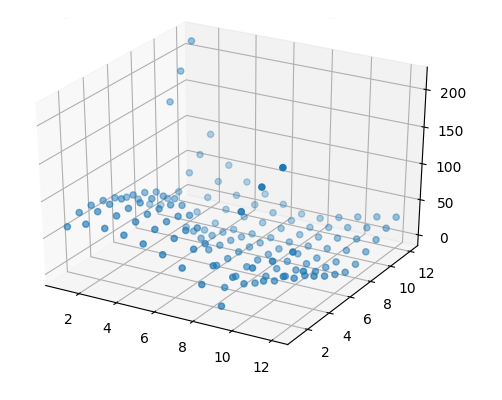
\includegraphics[scale=0.4]{learning/img/abs_plot_2_clean.png} &
		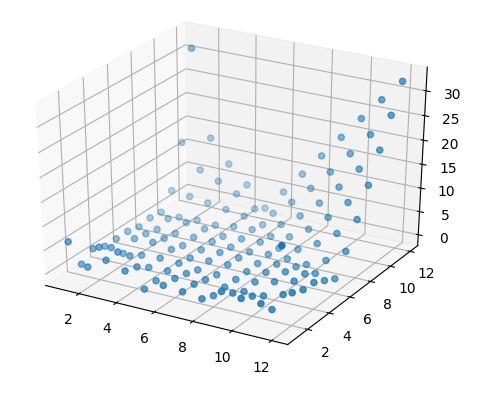
\includegraphics[scale=0.4]{learning/img/abs_plot_6_clean.png} \\
		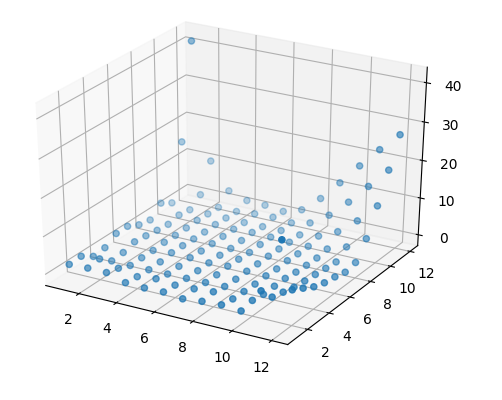
\includegraphics[scale=0.4]{learning/img/abs_plot_10_clean.png} &
		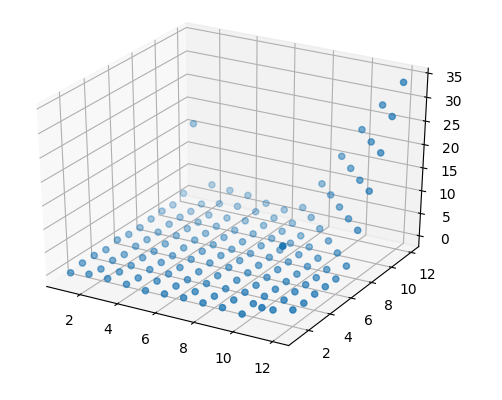
\includegraphics[scale=0.4]{learning/img/abs_plot_14_clean.png} \\				
	\end{tabular}
	\label{fig:mst_multiplicator_error}
	\caption{4 trainierte Neuronale Netzwerke mit 2 (\textit{oben links}), 6, 10 und 14 ( \textit{unten rechts}) Nodes im hidden Layer. Die blauen Punkte stellen sämtliche Kombinationen in X, Y auf dem Interval $[0,12)$ dar um zu verdeutlichen, wie sich der Fehler ausserhalb des trainierten Intervals $[0,10)$ entwickelt.}
\end{figure}

\begin{figure}
	\centering
	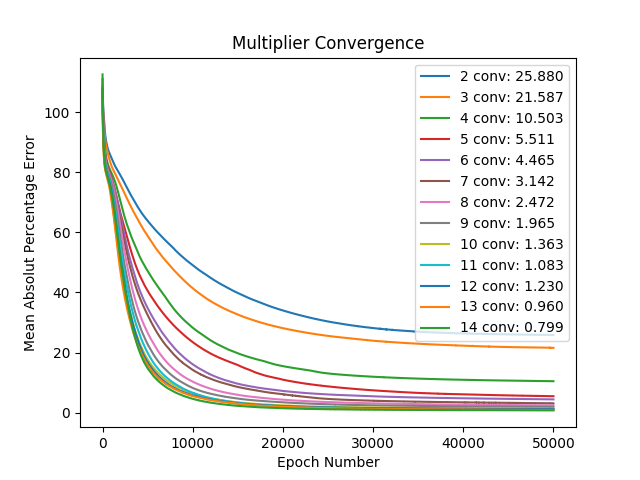
\includegraphics[scale=0.7]{learning/img/loss.png}
	\label{fig:mst_loss}
	\caption{Mit steigender Anzahl Neuronen im hidden Layer sinkt der relative Fehler gegen den im Training konvergiert wird.}
\end{figure}


